\section{Introduction}

\begin{figure}[tb]%
  \centering
  \label{fig:corner-types}
  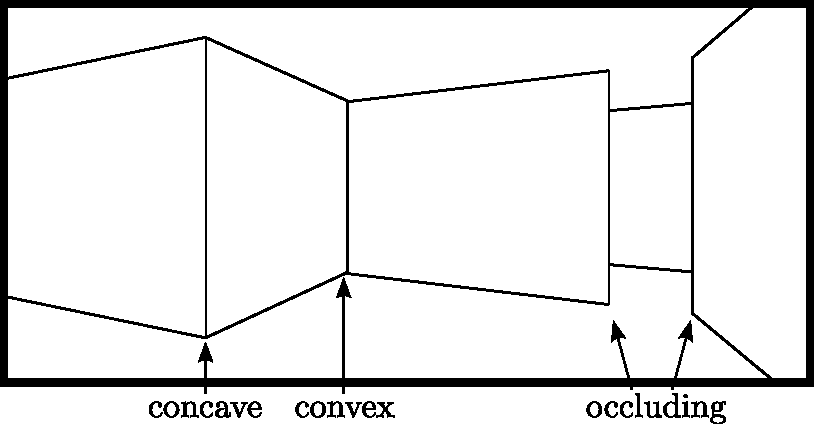
\includegraphics[width=0.3\textwidth]{corner-types}
  \hspace{0.1cm}
  \caption{Each corner in an indoor Manhattan environment can be
    categorized as concave, convex, or occluding. Each vertical line
    intersects exactly one wall segment. We denote the intersection of
    column $x$ with the top and bottom of the wall in that column
    $\PfAtX$ and the $\PcAtX$ respectively.}
\end{figure}

In this section we describe probabilistic models relating indoor
Manhattan model to observations. We consider three sensor modalities:
monocular image features, stereo features, and 3D point clouds. For
each we present a generative model relating observed features to the
Manhattan scene structure, which we denote $\Scene$. We show in each
case that the logarithm of the posterior $P(\Scene~|~X)$ be written as
a column--wise sum over a payoff function $\PixelPayoff(x,y)$ together
with a regularizer. This allows us to present a unified inference
algorithm in chapter \ref{chap:inference}, which efficiently solves
both maximum--apsteriori and maximum--likelihood inference for each
sensor modality, as well as for the combination of all three.

Rather than presenting a graphical model at the outset as in the
previous chapter, here we prefer to present models for each sensor
modality one--by--one to aid comprehension, then present the joint
model at the end.

%%%%%%%%%%%%%%%%%%%%%%%%%%%%%%%%%%%%%%%%%%%%%%%%%%%%%%%%%%%%%%%%%%%%%%
\section{Payoff Formulation}

In this section we describe a class of optimization problems that we
will refer to as \textit{payoff form}. Throughout the remainder of
this chapter it will become clear that a range of inference problems
in the context of indoor Manhattan scenes can be expressed in this
form, and in the following chapter it will become clear that this
particular formulation permits a general and efficient dynamic
programming solution.

Let $\SetOfScenes$ be the set of indoor Manhattan scenes in vertex
representation. Let $\Scene\in\SetOfScenes$ be a scene in vertex
representation and let $\Seam$ be the corresponding scene in
seam representation. 

A payoff function $\PixelPayoff: \Dom\cross\SetOfOrientations
\Mapto\Reals$ maps orientations $\Orient\in\SetOfOrientations$
together with integer pixel coordinates $\Pixel\in\Dom\subset\Ints^2$
to real numbers. The payoff for a scene $\Scene$ is defined in terms
of the seam representation,
\begin{equation}
  \label{eq:scene-payoff}
  \ScenePayoff(\Scene) = 
  \ScenePayoff(\Seam) =
  \sum_{j=1}^{\Width} \PixelPayoff(j,\seam_j,\WallOrient_j)
\end{equation}
where $\Seam = \{(\seam_j,\WallOrient_j)\}$. In cases where the payoff
function is independent of $\Orient_j$ we will write
\begin{equation}
  \PixelPayoff(\Pixel) = \PixelPayoff(\Pixel_x,\Pixel_y)
\end{equation}
Figure XXX shows several example of the seam over which this sum is
computed.

Note that the value of $\PixelPayoff(\Pixel)$ is \textit{not}
restricted in any way to dependence on the image evidence at pixel
$\Pixel$, nor even to a local region about $\Pixel$; indeed, the
payoff functions described in the following sections incorporate image
evidence from widely separated image regions.

Next we define a penalty function
$\ScenePenalty:\SetOfScenes\Mapto\Reals$ in terms of the vertex
representation,
\begin{equation}
  \label{eq:scene-penalty}
  \ScenePenalty(\Scene) = 
  \sum_{i=0}^{\NumWalls-1} \CornerPenalty(i;\Scene)
\end{equation}
where $\NumWalls$ is the number of walls contained in $\Scene$ and
$\CornerPenalty$ may be interpreted as a regulariser related to the
meeting between the $i$\th wall in $\Scene$ and its
successor. Finally, we define our objective
\begin{eqnarray}
  \label{eq:scene-objective}
  \Objective(\Scene) &=&
  \ScenePayoff(\Scene) - \ScenePenalty(\Scene)\\
  &=&
  \sum_{j=1}^{\Width} \PixelPayoff(j,\seam_j,\WallOrient_j) -
  \sum_{i=0}^{\NumWalls-1} \CornerPenalty(i;\Scene) ~.
\end{eqnarray}
which we will optimize as in
\begin{equation}
  \label{eq:opt-scene}
  \EstimatedScene = \argmax_{\Scene\in\SetOfScenes}\limits \Objective(\Scene) ~.
\end{equation}
Note that the objective $\Objective$ is defined partially in the scene
representation and partially in the vertex representation. This poses
no difficulty to evaluating the objective in the vertex representation
since we can readily obtain the seam representation via equation
\eqnref{seam-from-scene}. However, as discussed in
\secref{sec:seam-representation} the mapping from the vertex
representation to seam representation is not invertible, so the
objective above cannot be evaluated in the seam representation. For
this reason we will work in the vertex representation for the
presentation of the optimization algorithm in \chapref{inference}, but
for convenience we will work in seam representation to define the
payoff $\ScenePayoff$, which is the topic of the remainder of this
chapter.

%%%%%%%%%%%%%%%%%%%%%%%%%%%%%%%%%%%%%%%%%%%%%%%%%%%%%%%%%%%%%%%%%%%%%%
\section{Model For Estimating Manhattan Homology}

%%%%%%%%%%%%%%%%%%%%%%%%%%%%%%%%%%%%%%%%%%%%%%%%%%%%%%%%%%%%%%%%%%%%%%
\section{Prior On Scenes}

We turn first to the prior on models, $P(\Scene~|~\Penalties)$, which
is governed by the hyper--parameters $\Penalties$. As discussed in
\secref{corner-categories}, corners between successive walls can be
clasified as concave, convex, and occluding. Let $n_1, n_2,$ and $n_3$
be the number of corners in $\Scene$ of each category
respectively. Our prior on scenes is a geometric distribution in
$\vect{n}$,
\begin{eqnarray}
  \label{eq:scene-prior}
  P(\Scene ~|~ \Penalties) &=& \frac{1}{Z} 
    {\PenaltyConc}^{n_1} {\PenaltyConv}^{n_2} {\PenaltyOccl}^{n_3}\\
  Z &=& \frac{\mu(n_1,n_2,n_3)}{(1-\PenaltyConc)(1-\PenaltyConv)(1-\PenaltyOccl)}~,
\end{eqnarray}
where $\mu(n_1,n_2,n_3)$ measures the number of scenes with a certain
number concave, convex, and occluding corners. The prior
\eqnref{scene-prior} may be interpreted as a process in which $n_i$ is
determined by the number of times that a biased coin comes up heads
before the first observed tails, where the probability of heads in
each round is $\Penalty_i$. Our choice of \eqnref{scene-prior} is
motivated by the desire to penalize scenes for additional complexity,
which we take to correspond roughly to the number walls. We discuss
alternative priors, and some of the problems they raise during
inference, in \secref{alternative-priors}.

Taking logarithms yields
\begin{equation}
  \label{eq:log-scene-prior}
  \log P(\Scene ~|~ \Penalties) =
    -\log Z +
    n_1\log\PenaltyConc + 
    n_2\log\PenaltyConv + 
    n_3\log\PenaltyOccl~.
\end{equation}
Comparison with \eqnref{scene-penalty} suggests the following
penalty function:
\begin{equation}
  \label{eq:corner-penalty}
  \CornerPenalty(i;\Scene) = 
  \begin{cases}
    \log \PenaltyConc, & \mbox{if corner $i$ is concave} \\
    \log \PenaltyConv, & \mbox{if corner $i$ is concex} \\
    \log \PenaltyOccl, & \mbox{if corner $i$ is occluding.} \\
  \end{cases}
\end{equation}
The three cases can be decided by the algorithm described in
\secref{corner-categories}. Note that the scene penalty differs from
the log--posterior by a additive constant,
\begin{equation}
  \ScenePenalty(\Scene) = \log P(\Scene ~|~ \Penalties) + \log Z
\end{equation}
but we will ignore this term since our ultimate goal is the
optimization expressed in \eqnref{opt-scene}.

%%%%%%%%%%%%%%%%%%%%%%%%%%%%%%%%%%%%%%%%%%%%%%%%%%%%%%%%%%%%%%%%%%%%%%
\section{Photometric Sensor Model}

We now introduce a probabilistic model relating indoor Manhattan
scenes to observed image features. We begin with the single--view
scenario in which we observe a feature vector $\Feature\in\Reals^n$ at
each pixel $\Pixel$. 

\begin{figure}[tb]
  \centering
  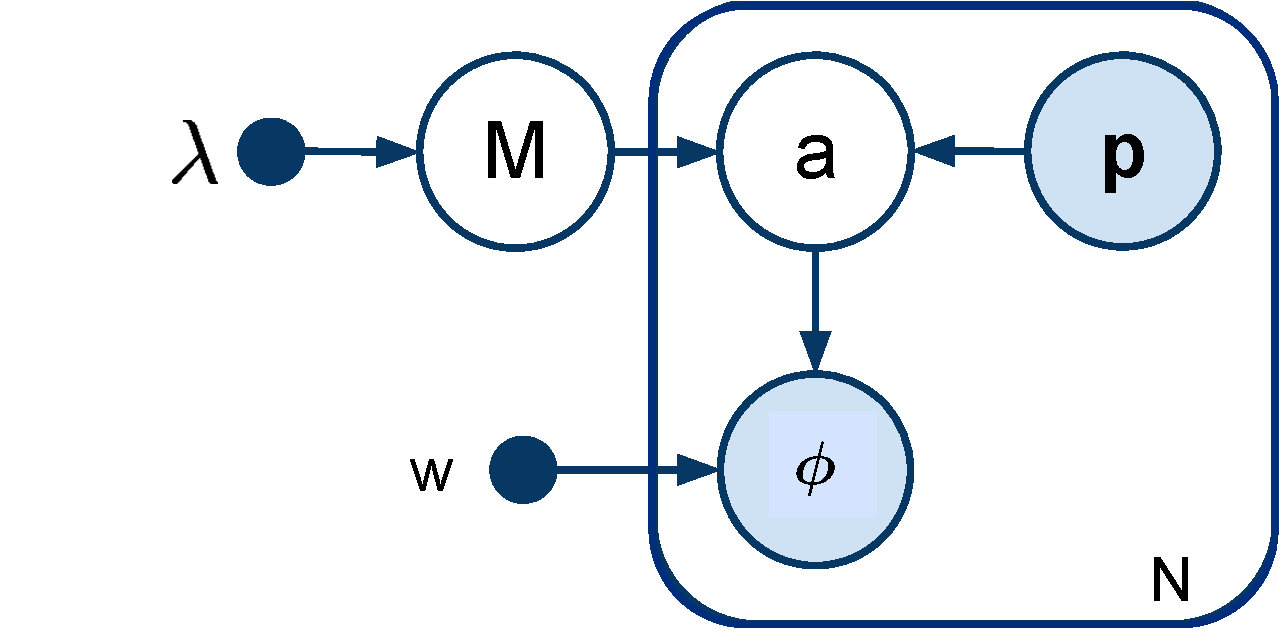
\includegraphics[width=0.6\textwidth]{monocular-gm}
  \caption{The graphical model relating scenes $\Scene$ to monocular
    image features $\Feature$. $\Pixel=(x,y)$ is a pixel location and
    $a$ is the orientation predicted (deterministically) by $\Scene$
    at $\Pixel$.}
  \label{fig:monocular-gm}
\end{figure}

We assume the graphical model shown in \figref{monocular-gm}. The
generative process begins by sampling a scene $\Scene$, then samples
pixels $\Pixel$ and computes their orientation
$\Orient\in\Orientations$ (\cf
\algref{computing-from-scene}), which is deterministic given $\Scene$
and is included in the graphical model for notational convenience
only. Finally a feature $\Feature$ is sampled from a distribution that
is conditionally independent of $\Scene$ given $\Orient$.

We assume a exponential--family likelihood for pixel features,
\begin{equation}
  \label{eq:pixel-likelihood}
  P(\Feature ~|~ \Orient) \propto
    \exp(\PixelModel_\Orient \cdot \Feature) ~.
\end{equation}

Denoting the set of all observed pixel
features $\Features$, pixels $\Pixels$, and orientations $\Orients$,
the joint distribution is
\begin{equation}
  P(\Features, \Pixels, \Orients, \Scene, \Penalties, \PixelModel) =
    P(\Scene ~|~ \Penalties) 
    \prod P(\Pixel_i)
          P(\Orient_i ~|~ \Scene, \Pixel_i)
          P(\Feature_i ~|~ \Orient_i, \PixelModel) ~.
\end{equation}
We do not model the distribution $P(\Pixel_i)$ and for the remainder
of this section it may be assumed that all probabilities are
conditioned on this quantity.

We now derive MAP inference. The likelihood for $\Scene$ is
\begin{equation}
  \label{eq:photometric-lik-full}
  P(\Features ~|~ \Scene) \propto 
  \int
    \prod_i P(\Feature_i ~|~ \Orient_i) 
            P(\Orient_i ~|~ \Scene)
  \intd \Orients ~.
\end{equation}
In the integration over the latent variables $\Orient_i$ the only
non--zero term is the one for which all $\Orient_i$ are equal to that
predicted by \algref{computing-from-scene}. Therefore, denoting by
$\PredictedOrient_i$ the orientation output by
\algref{computing-from-scene} for pixel $\Pixel_i$ under $\Scene$ we
have
\begin{equation}
  \label{eq:photometric-lik}
  P(\Features ~|~ \Scene) \propto
    \prod_i P(\Feature_i ~|~ \PredictedOrient_i) ~.
\end{equation}
Taking logarithms gives
\begin{equation}
  \label{eq:photometric-loglik}
  \log P(\Features ~|~ \Scene) =
    \sum_i \log P(\Feature_i ~|~ \Orient_i^*) + c
\end{equation}
where $c$ corresponds to the constant of proportionality in
\eqnref{photometric-lik}, which we henceforth drop since it makes no
difference to the optimization to come. 

At this point we use the crucial observation of
\secref{col-decomposability} that the orientations
$\PredictedOrient_i$ can is functionally dependent only on the pair
$(\seam_j,\WallOrient_j)$ for the column $j$ containing
$\Pixel_i$. Let $\ComputedOrient(x,y;\seam_j,\WallOrient_j)$ be the
orientation output by \algref{computing-from-scene} for pixel $(x,y)$
under the hypothesis $(\seam_j,\WallOrient_j)$. We define
\begin{equation}
  \label{eq:mono-payoffs}
  \MonoPayoff(x,y,\WallOrient) = \sum_{r=0}^H \log 
    P(\Feature_{xr} ~|~ \ComputedOrient(x,r;y,\WallOrient)~)
\end{equation}
where the double--subscript in $\Feature_{xr}$ is a result of
separately indexing rows and columns in \label{eq:mono-payoffs}. 

Now consider the scene payoff,
\begin{eqnarray}
  \ScenePayoff(\Scene) &=& 
    \sum_{j=0}^W \MonoPayoff(j, \seam_j, \WallOrient_j) \\
  &=& 
    \sum_{j=0}^W \sum_{r=0}^H \log
      P(\Feature_{jr} ~|~ \ComputedOrient(j,r;\seam_j,\WallOrient_j)~)\\
  &=&
    \log P(\Features ~|~ \Scene) - c  ~,
\end{eqnarray}
which is simply the log--likelihood \eqnref{photometric-loglik}.

\subsection{Features}

RGB

HSV

Gabor

\subsubsection{Line Sweeps}
\label{sect:orient-est}

This feature adapts the simple and efficient line--sweep algorithm of
Lee \etal \cite{Lee09}, which produces a partial labelling of the
image in terms of the three Manhattan surface orientation labels
(corresponding to the three Manhattan orientations in the image). 

%%%%%%%%%%%%%%%%%%%%%%%%%%%%%%%%%%%%%%%%%%%%%%%%%%%%%%%%%%%%%%%%%%%%%%
\section{Multiple--View Sensor Model}

\begin{figure}[tb]
  \centering 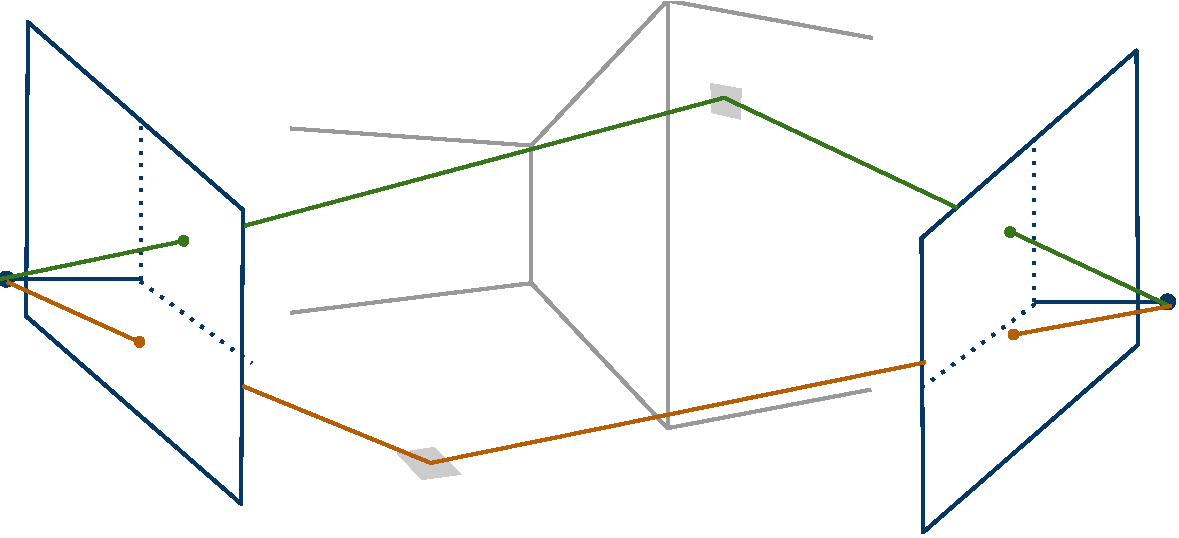
\includegraphics[width=0.8\textwidth]{backproject}
  \caption{Pixel correspondences across multiple views are computed by
    back--projection onto the model $\Scene$ followed by re--projection into
    auxiliary views.}
  \label{fig:backproject}
\end{figure}
We now formulate the payoff function $\StereoPayoff$ for the case that
multiple views of the scene are available. Intuitively, we treat
inference in this settings as follows. We consider models $\Scene$ in
terms of their projection into $\Image_0$. We explained in
\secref{model} that models parametrized in image coordinates specify
unique 3D models. Any hypothesized model can therefore be
re--projected into the auxiliary views, giving pixel--wise
correspondences between frames (\cf \figref{backproject}). From this
we compute a photo--consistency measure $\pc(\cdot)$, which provides
the likelihood $P(\StereoData ~|~ \Scene)$. The prior remains as in
\eqnref{scene-prior}.

Optimizing over photo--consistency has been standard in the stereo
literature for several decades \cite{Scharstein01}; our contribution
is to show that (i) in the particular case of indoor Manhattan models,
photo--consistency can be expressed as a payoff matrix; (ii) that we
can therefore perform efficient and exact global optimization; and
(iii) that this fits naturally within a Bayesian framework alongside
monocular and 3D features.

We assume that there one frame is identified as the base frame
$\Image_0$; the remaining $\NumViews$ frames are denoted
$\Image_1,\ldots,\Image_{\NumViews}$. We assume that all cameras are fully
calibrated with the action of the $i$\th camera on a 3D points $X$
being
\begin{equation}
  \CamMatrix_i (\CamR_i X + \CamTr_i) ~.
\end{equation}
We normalize images intensities to zero mean and unit variance.

In \secref{metric-recovery} we showed how to convert a scene in vertex
representation to a 3D reconstruction. Since all cameras are
calibrated we use such a reconstruction to re--project any pixel
$\Pixel$ in the base view into any auxiliary view, as illustrated in
\figref{backproject}. Let $\AuxPixel_k(\Pixel;\Scene)$ be the
re--projection of $\Pixel$ into view $k$ via the scene hypothesis
$\Scene$. Let each pixel $\Pixel_i$ in the base image be associated
with a feature vector $\Feature_i\in\Reals^n$ and let each pixel
$\AuxPixel_{ki}$ in the $k$\th auxiliary view be simirlarly associated
with a feature $\AuxFeature_{ki}\in\Reals^n$. Let $\Features$ be the
set of all features in the base view and let $\AuxFeatures_k$ be the
set of all features in the $k$\th auxiliary view. Finally, let
\begin{equation}
  \ComputedAuxFeature_k(\Pixel_i;\Scene) =
  \AuxFeature(\AuxPixel_k(\Pixel_i;\Scene))
\end{equation}
be the feature associated with the reprojection of $\Pixel_i$ into the
$k$\th auxiliary view under the scene hypothesis $\Scene$. Then the
likelihood for $\Scene$ under our model is
\begin{equation}
  P(\Features,\AuxFeatures_1,\ldots,\AuxFeatures_K ~|~ \Scene) =
    \prod_i \prod_{k=0}^{\NumViews} 
      P(\Feature_i, \ComputedAuxFeature_k(\Pixel_i;\Scene) ~|~ \StereoCov)~.
\end{equation}
and the feature likelihood is a zero--mean Gaussian, which is standard in
the literature \cite{Scharstein01}:
\begin{equation}
  P(\Feature_i, \ComputedAuxFeature_k(\Pixel_i;\Scene) ~|~ \StereoCov)
   = \NormalDistr(\Feature_i-\ComputedAuxFeature_k(\Pixel_i;\Scene); \StereoCov)
\end{equation}

Taking logarithms we recognise a simple sum over pixel--wise
photo--consistency terms,
\begin{equation}
  \label{eq:stereo-loglik}
  \log P(\Features,\AuxFeatures_1,\ldots,\AuxFeatures_{\NumViews}
            ~|~ \Scene) =
  \sum_i \sum_{k=0}^{\NumViews} 
    \|\Feature_i-\ComputedAuxFeature_k(\Pixel_i;\Scene)\|_{\StereoCov}
   +c
\end{equation}

\begin{figure}[tb]
  \centering 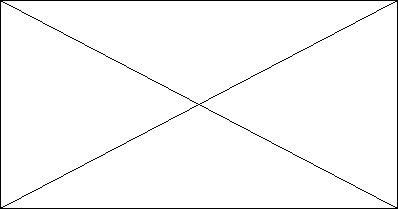
\includegraphics[width=0.8\textwidth]{placeholder}
  \caption{TODO: Reprojected image columns.}
  \label{fig:reprojected-columns}
\end{figure}

We now write equation \eqnref{stereo-loglik} in payoff form. To this
end we leverage the observation made in \secref{col-decomposability}
that the depth of a pixel $\Pixel$ under a scene hypothesis $\Scene$
is functionally dependent only on the pair $(\seam_j,\WallOrient_j)$
for the column $j$ containing $\Pixel$. Let
$\ComputedDepth(\Pixel;\seam_j)$ be the depth of $\Pixel$ under
hypothesis $\seam_j$, as output by \algref{seam-depth-orient}.

Furthermore, re--projecting a pixel into an auxiliary view requires
only the depth $\Depth_i$ of the scene at the pixel together with the
camera parameters. Therefore we can identify the correspondences for
any pixel $\Pixel$ in all auxiliary views from the value $\seam_j$
alone. Specifically, the re--projection of $\Pixel$ into the $k$\th
view under the hypothesis $\seam_j$ is
\begin{equation}
  \AuxPixel_k(\Pixel;\seam_j) = \CamMatrix_k (\CamR_k X_i + \CamTr_k)
\end{equation}
where
\begin{equation}
  X_i = 
  \CamR_0^{-1} \bigl(
    \bar{\Depth}(\Pixel;\seam_j) \CamMatrix_0^{-1} \Pixel - \CamTr_0
  \bigr) ~.
\end{equation}
We can now re--write the correspondence function
$\ComputedAuxFeature_{ki}$ in terms of $\seam_j$ alone,
\begin{equation}
  \ComputedAuxFeature_k(\Pixel;\seam_j) = 
    \AuxFeature(\AuxPixel_k(\Pixel;\seam_j)) ~.
\end{equation}
Finally, the payoff function is
\begin{equation}
  \label{eq:stereo-payoffs}
  \StereoPayoff(x,y) = \sum_{r=0}^H \sum_{k=1}^{\NumViews}
    \| \Feature_{xr} - \ComputedAuxFeature_k([x,r]^T;y) \|_\Sigma
\end{equation}
where as in \eqnref{mono-payoffs} we have switched to a separate
indexing scheme for rows and columns, so $\Feature_{xy}$ is the
feature for the pixel at $(x,y)$ and $\ComputedAuxFeature_k(x,r;y)$
the the feature for the reprojection of $(x,r)$ into the $k$\th view
under the hypothesis $\seam_j=y$.

Substituting \eqnref{stereo-payoffs} into \eqnref{scene-payoff},
\begin{eqnarray}
  \ScenePayoff(\Scene) &=& 
    \sum_{j=0}^W \StereoPayoff(j,\seam_j)\\
  &=&
    \sum_{j=0}^W \sum_{r=0}^H \sum_{k=1}^{\NumViews}
    \| \Feature_{jr} - \ComputedAuxFeature_k([j,r]^T;\seam_j) \|_\Sigma\\
  &=&
    \log P(\Features,\AuxFeatures_1,\ldots,\AuxFeatures_{\NumViews}
             ~|~ \Scene) - c
\end{eqnarray}

\subsection{An Alternative View}

% SPACE: remove para below
Our approach could also be cast as solving the general stereo problem
in terms of disparity maps, where in place of priors based on various
pixel--wise smoothness constraints, our prior is \eqnref{scene-prior}
for disparity maps corresponding to valid indoor Manhattan
reconstructions, and zero otherwise. Inference under this model would
be intractible if cast directly in terms of disparity maps because
determining whether a given disparity map corresponds to some indoor
Manhattan reconstruction is difficult. Nevertheless, our approach
shows that by re--parametrising in the vertex representation
\eqnref{vertex-repr} the problem becomes tractible.

Note that the column--wise decomposition \eqnref{stereo-payoffs}
neither commits us to optimizing over columns independently, nor to
ignoring interactions between columns. Indeed by inspecting the
graphical model in \figref{stereo-gm} one sees immediately that our
model assumes no independence between image columns (only conditional
independence given $\Scene$). Such correlations come into effect when
we optimize over the full payoff matrix in \chapref{inference}, and
our results will show that widely separated image regions often
interact strongly. The derivations in this section follow deductively
from the indoor Manhattan assumption; the only approximation is the
following.

\subsection{Occlusions}. We have ignored self--occlusions in
\eqnref{stereo-likelihood}. For short baselines, such as frames
sampled over a few seconds from a moving camera, this is unproblematic
since indoor environments tend to be mostly convex from any single
point of view. Even in highly non--convex environments our system
achieves excellent results by integrating 3D and monocular features,
and enforcing strong global consistency, as will be shown in
our experimental section. Further discussion of this issue is in the
final section of this chapter.

%%%%%%%%%%%%%%%%%%%%%%%%%%%%%%%%%%%%%%%%%%%%%%%%%%%%%%%%%%%%%%%%%%%%%%
\section{Point Cloud Sensor Model}

\begin{figure}[tb]
  \centering
  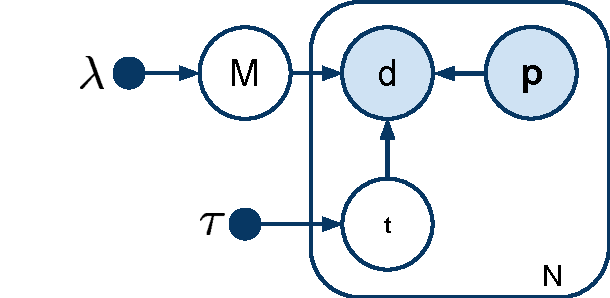
\includegraphics[width=0.6\textwidth]{3d-gm}
  \caption{The graphical model relating indoor Manhattan models to 3D
    points. The hidden variable $t$ indicates whether the point is
    inside, outside, or coincident with the model.}
  \label{fig:3d-gm}
\end{figure}

In this section we explore the context in which a 3D point cloud is
available during inference. The point clouds generated by
structure--from--motion systems are typically too sparse for direct
reconstruction, but can provide useful cues alongside monocular and
stereo data.

\begin{figure}[tb]
  \centering 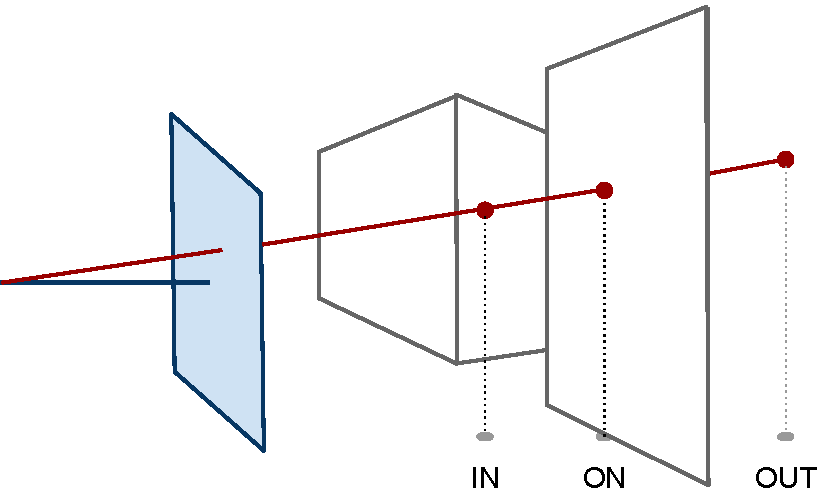
\includegraphics[width=0.8\textwidth]{point-projs}
  \caption{Depth measurements $d_i$ might be generated by a surface in
    our model (represented by $t_i=\ON$) or by an object inside or
    outside the environment (in which case $t_i=\IN,\OUT$
    respectively).}
  \label{fig:point-projs}
\end{figure}


%For each pixel $\Pixel_i$ a depth measurement $d_i$ is made. The
%relationship between $d$ and the model $M$ is determined by a hidden
%variable $t\in\{\textsf{IN},\textsf{ON},\textsf{OUT}\}$, which is
%interpreted as follows. Let $\DepthAtPGivenModel$ be the true depth of
%the model $\Scene$ in the direction $\Pixel$. If $t=\textsf{IN}$ then
%$\Depth$ corresponds to an object inside the room,

Our graphical model for 3D data is depicted in \figref{3d-gm}. The
model $\Scene$ is sampled according to the prior \eqnref{scene-prior},
then depth measurements $d_i$ are generated for pixels
$\Pixel_i$. Many such measurements will correspond to clutter or
measurement errors, rather than to the walls represented by
$\Scene$. Our model captures this uncertainty explicitly through
the latent variable $t_i$, which has following interpretation. If
$t_i=\ON$ then $d_i$ corresponds to some surface represented
explicitly in $\Scene$. Otherwise, either $t_i=\IN$, meaning some
clutter object within the room was measured, or $t_i=\OUT$, in which
case an object outside the room was measured, such as through a
window. The likelihoods we use are
\begin{align}
  \label{eq:x-inside}
  P(\Depth~|~\Pixel,\Ind=\textsf{IN},\Scene) &=
  \begin{cases}
    \alpha, & \mbox{if } 0 < \Depth < \DepthAtPGivenModel \\
    0, & \mbox{otherwise} \\
  \end{cases} \\
  \label{eq:x-outside}
  P(d~|~\Pixel,\Ind=\textsf{OUT},\Scene) &=
  \begin{cases}
    \beta, & \mbox{if } \DepthAtPGivenModel < \Depth < \Dmax \\
    0, & \mbox{otherwise} \\
  \end{cases} \\
  P(\Depth ~|~ \Pixel,\Ind=\textsf{ON},\Scene) &=
  \NormalDistr(\Depth~;~\DepthAtPGivenModel,\sigma) ~.
\end{align}
where $\alpha$ and $\beta$ are determined by the requirement that the
probabilities sum to $1$ and $\DepthAtPGivenModel$ denotes the depth
predicted by $\Scene$ at $\Pixel$. We compute likelihoods on $\Depth$ by
marginalizing over $\Ind$,
\begin{align}
  \label{eq:3d-likelihood}
  P(\Depth~|~\Pixel,\Scene,\IndModel) &=
   \sum_{\Ind} P(\Depth~|~\Pixel,\Scene,\Ind) P(\Ind~|~\IndModel)
  ~.
\end{align}
where $P(\Ind~|~\IndModel)$ is a categorical distribution with
parameters $\tIN$, $\tOUT$, and $\tON$. Equation
\eqnref{3d-likelihood} can be readily evaluated for any $\Depth$ and
$\Pixel$ since the sum is over just the three possible values for
$\Ind$. Denoting the set of all depth measurements $\Depths$, the full
likelihood for $\Scene$ is
\begin{eqnarray}
  \label{eq:depth-loglik}
  P(\Depths ~|~ \Pixels,\Scene) &=&
    \prod_i P(\Depth_i ~|~ \Pixel_i,\Scene)\\
  \log P(\Depths ~|~ \Pixels,\Scene) &=&
    \sum_i \log P(\Depth_i ~|~ \Pixel_i,\Scene)
\end{eqnarray}
We now utilise the same observation as we did in the previous section,
namely that the depth at $\Pixel$ is functionally dependent only on
the seam pair in the column containing $\Pixel$. Retaining the
notation under which $\ComputedDepth(\Pixel;\seam_j)$ is the depth at
$\Pixel$ computed by \algref{seam-depth-orient} for $\Scene$, we
define the payoff function
\begin{equation}
  \label{eq:depth-payoffs}
  \DepthPayoff(x,y) = 
  \sum_{i\in\Depths_x} \log P(\Depth_i~|~\Pixel_i,\ComputedDepth(\Pixel_i;y))
\end{equation}
where $\Depths_x$ contains indices for all depth measurements in
column $x$. We verify that \eqnref{depth-payoffs} does in fact
correspond to the log--likelihood \eqnref{depth-loglik} by
substituting the above into \eqnref{scene-payoff}, giving
\begin{eqnarray}
  \ScenePayoff(\Scene) &=& 
    \sum_{j=0}^W \DepthPayoff(j,\seam_j)\\
  &=&
    \sum_{j=0}^W \sum_{i\in\Depths_j} 
    \log P(\Depth_i~|~\Pixel_i,\ComputedDepth(\Pixel_i;\seam_j)~)\\
  &=&
    \log P(\Depths ~|~ \Pixels, \Scene)~.
\end{eqnarray}

%%%%%%%%%%%%%%%%%%%%%%%%%%%%%%%%%%%%%%%%%%%%%%%%%%%%%%%%%%%%%%%%%%%%%%
\section{Joint Model}
We combine photometric, stereo, and 3D data into a joint model by
assuming conditional independence given $\Scene$,
\begin{equation}
  P(\Observations_{\textsf{mono}}, \Observations_{\textsf{stereo}}, \Observations_{\textsf{3D}} ~|~ \Scene)
  =
    P(\Observations_{\textsf{mono}} ~|~ \Scene)
    P(\Observations_{\textsf{stereo}} ~|~ \Scene)
    P(\Observations_{\textsf{3D}} ~|~ \Scene) ~.
  \label{eq:full-posterior}
\end{equation}
Taking logarithms leads to summation over payoffs,
\begin{equation}
  \log P(\Observations_{\textsf{mono}}, \Observations_{\textsf{stereo}}, \Observations_{\textsf{3D}} ~|~ \Scene)
  = \ScenePayoff_{\textsf{joint}}(\Scene)
\end{equation}
where
\begin{equation}
  \JointPayoff(\Pixel) =
  \MonoPayoff(\Pixel) + 
  \StereoPayoff(\Pixel) +
  \DepthPayoff(\Pixel) ~.
\end{equation}
Finally, the log posterior is
\begin{equation}
\begin{split}
  \log P(\Scene ~|~ \Observations_{\textsf{mono}}, \Observations_{\textsf{stereo}}, \Observations_{\textsf{3D}})
  & \propto
    \log P(\Observations_{\textsf{mono}} ~|~ \Scene)
    +\log P(\Observations_{\textsf{stereo}} ~|~ \Scene) \\
  & \quad + \log P(\Observations_{\textsf{3D}} ~|~ \Scene) + \log P(\Scene)\\
  & = \ScenePayoff_{\textsf{joint}}(\Scene) - \ScenePenalty(\Scene)
\end{split}
\end{equation}

We can now cast maximum--likelihood and maximum--aposteriori inference
in the form \eqnref{scene-objective},
\begin{eqnarray}
  \EstimatedScene_{\mbox{\tt ML}} &=& 
    \argmax_{\Scene\in\SetOfScenes}\limits~
    \ScenePayoff_{\textsf{joint}}(\Scene)\\
  \EstimatedScene_{\mbox{\tt MAP}} &=& 
  \argmax_{\Scene\in\SetOfScenes}\limits~
  \ScenePayoff_{\textsf{joint}}(\Scene) - \ScenePenalty(\Scene)\\
\end{eqnarray}

%%%%%%%%%%%%%%%%%%%%%%%%%%%%%%%%%%%%%%%%%%%%%%%%%%%%%%%%%%%%%%%%%%%%%%
\section{Discussion}

Lighting invariants and normalization for stereo

Joint multiple view models - joint gaussian?

\subsection{Extension: using orientation information for stereo}

\subsection{EM for Occlusion Resolution}

%%%%%%%%%%%%%%%%%%%%%%%%%%%%%%%%%%%%%%%%%%%%%%%%%%%%%%%%%%%%%%%%%%%%%%
\section{Conclusion}
We have presented a Bayesian framework for scene understanding in the
context of a moving camera. Our approach draws on the indoor Manhattan
assumption introduced for monocular reasoning and we have shown that
techniques from monocular and stereo vision can be integrated with 3D
data in a coherent Bayesian framework.

In future work we intend to use indoor Manhattan models to reason
about objects, actions, and scene categories. We also intend to
investigate structural SVMs for learning parameters, which may allow
us to relax the conditional independence assumptions between sensor
modalities.
